In cui si spiega brevemente il processo di installazione del software su di un server di produzione.

\section{Struttura}
Il sistema così realizzato finora consta di due componenti:
\begin{itemize}
    \item \textbf{SPA / frontend applicativo}: interagisce con il backend tramite protocollo HTTP.
    \item \textbf{REST API / backend applicativo}: risponde alle richieste del frontend attraverso l'interfacciamento con la socket UNIX del sistema Greenbone.
\end{itemize}
Dall'ultimo punto segue che la REST API e l'istanza del sistema Greenbone devono trovarsi necessariamente sullo stesso server. In alternativa, almeno il demone GVM deve essere presente sullo stesso server.

La SPA di frontend tuttavia può trovarsi anche su di un server differente e interagire con l'API del backend Flask tramite protocollo HTTP. Questo può aprire interessanti possibilità di ottimizzazione se si vuole usare delle CDN o altri strumenti di edge computing.

Nel nostro caso specifico tuttavia entrambi i componenti sono stati installati sullo stesso server, per pura semplicità.

\section{Containerizzazione}
L'installazione delle componenti e la loro integrazione con il sistema Greenbone sono state entrambe realizzate attraverso Docker (e più nello specifico, Docker Compose).

Infatti, come già detto in \ref{greenbone-community-containers}, Greenbone mette a disposizione un'installazione ufficiale e supportata dell'intero framework attraverso la piattaforma di Docker Compose. Per un ambiente di produzione questa strategia garantisce riproducibilità e affidabilità, ma anche un aggiornamento in generale estremamente semplice, per il quale basta distruggere i container esistenti, aggiornare le immagini di Docker e ricreare i container.

Questo di fatto guida il processo di installazione verso una strategia semplice, ma efficace: \emph{dockerizzare} (ovvero realizzare un Dockerfile) entrambe le componenti realizzate per questo progetto (frontend e backend) e interconnetterle in Docker Compose tramite due container appositi.

\subsection{Immagine del backend}
\label{deployment-backend}
Il backend è stato trasposto in un container Docker secondo il seguente procedimento, seguendo a grandi linee il seguente \texttt{Dockerfile}:
\begin{figure}[!h]
    \centering
    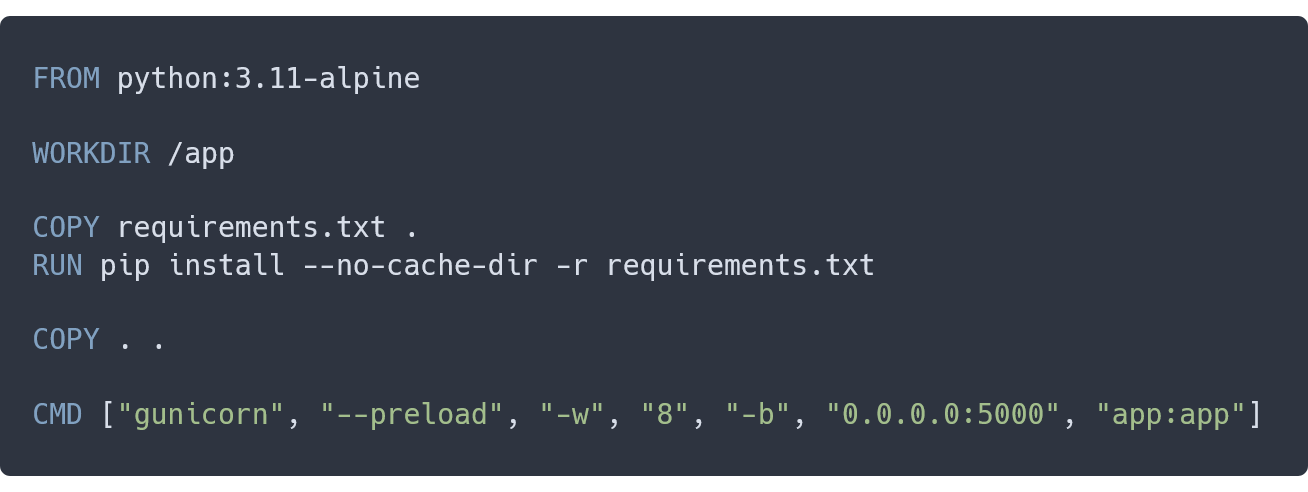
\includegraphics[width=0.8\textwidth]{img/dockerfile-backend.png}
    \caption{Dockerfile usato per l'immagine del backend Flask}
\end{figure}
\begin{enumerate}
    \item Si parte da un'immagine di base della versione di Python utilizzata durante lo sviluppo del progetto. La versione \texttt{alpine} garantisce un minor consumo di spazio di disco\footnote{Le immagini \texttt{alpine} si riferiscono a immagini Docker basate su \textbf{Alpine Linux}, una distribuzione Linux leggera e minimalista. Alpine è progettata per essere piccola, sicura e semplice, il che la rende una scelta popolare per la creazione di container Docker, dove il sistema operativo richiesto tipicamente deve eseguire non più di un'applicazione. Gran parte della riduzione di dimensioni è dovuta all'uso di \texttt{musl} come libreria C al posto della più famosa \texttt{glibc}. \texttt{musl} infatti è molto più piccola e coesa, ma c'è sempre il rischio che alcune applicazioni non funzionino come dovrebbero in un ambiente Alpine, siccome si aspettano la libreria \texttt{glibc} che ormai è uno standard di fatto in ambiente Linux.}.
    \item Nell'immagine viene copiato solo il file delle dipendenze (\texttt{requirements.txt}), che vengono installate con \texttt{pip}. In questo modo si può sfruttare al massimo il \emph{caching} dei layer di Docker.
    \item Il codice viene copiato nella sua totalità.

    In questo passaggio viene anche copiato nell'immagine il file \texttt{.env}, che chiaramente deve essere creato e configurato non essendo stato aggiunto al sistema di controllo versione.

    In particolare, il file dovrebbe essere configurato con:
    \begin{itemize}
        \item Una chiave di crittografia, necessaria siccome usiamo i cookie di Flask. Questa può essere creata facilmente e in sicurezza usando un interprete di Python per generarla in modo crittograficamente sicuro.
        \item Il numero massimo di IP configurabili per ogni bersaglio in GVM.
        
        Di default un'installazione del framework Greenbone è configurata con un massimo di $2^{12}-1$ IP per bersaglio, ma questa soglia può essere alzata in un secondo momento sino ad un limite di $\approx 70000$ che essendo $> 2^{16}$ permette almeno di configurare anche subnet $/16$ in notazione CIDR, che sono comuni in molti contesti aziendali.
        \item Gli UUID dei ruoli configurati come da schema descritto in \ref{roles}. Questi possono essere facilmente ottenuti tramite GSA.
        \item IP, porta, DB e password dell'istanza Redis. Siccome stiamo usando Docker Compose l'istanza di Redis di fatto è ospitata su un container dedicato, quindi la porta sarà quella usata dal container (che può essere tranquillamente quella di default senza problemi di sicurezza, visto che non sarà pubblicata al di fuori della macchina) mentre l'IP è il nome dato al container che nelle funzionalità di rete offerte da Docker funge da hostname.
    \end{itemize}
    \item Come entrypoint si utilizza il web server WSGI\footnote{\textbf{Web Server Gateway Interface} è un'interfaccia standard tra web server e applicazioni web scritte in Python. Molti dei più famosi framework Python come Flask e Django aderiscono allo standard WSGI, e pertanto possono essere facilmente installati grazie a web server anch'essi compatibili con WSGI. Gunicorn è uno dei più famosi server web di questo tipo, e può essere installato come una semplice dipendenza \texttt{pip}.} \textbf{Gunicorn}, configurato per precaricare il codice precedentemente al fork dei processi worker.
\end{enumerate}

\subsection{Immagine del frontend}
Il frontend invece segue il seguente \texttt{Dockerfile}:
\begin{figure}[!h]
    \centering
    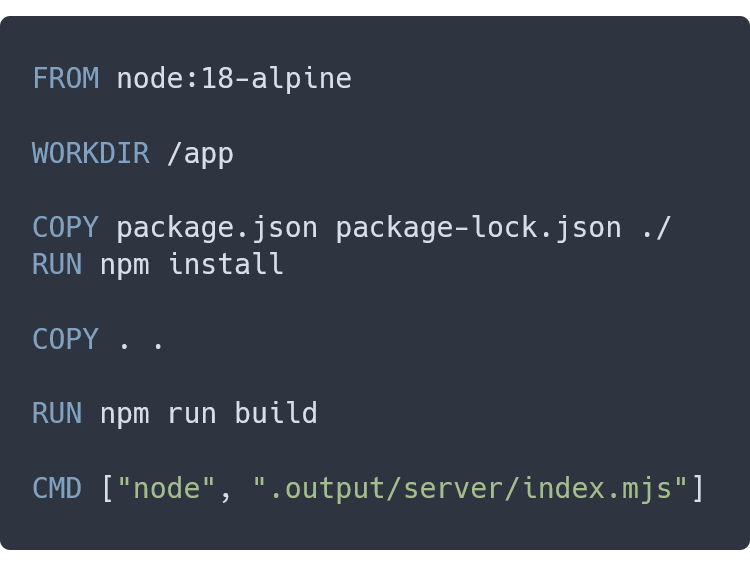
\includegraphics[width=0.5\textwidth]{img/dockerfile-frontend.png}
    \caption{Dockerfile usato per l'immagine del frontend Nuxt}
\end{figure}
\begin{enumerate}
    \item Come immagine di base si è scelta una \texttt{node} della versione corrispondente a quella usata nell'ambiente di sviluppo.
    \item Nell'immagine vengono copiati i file \texttt{package.json} e \texttt{package.lock}, per poi installare le dipendenze con \texttt{npm}.
    \item Viene copiato il resto del codice. Anche qua viene fatto questo passaggio ulteriore per sfruttare il \emph{caching} delle immagini Docker. Inoltre, viene copiato il file \texttt{.env}, che deve essere creato e configurato con l'unica variabile rilevante: l'endpoint dell'API. Si noti che in questo caso è necessario fornire un endpoint visibile dal web, siccome questo indirizzo sarà usato per le richieste fatte dal client Fetch di Nuxt, che non funzionano in ambiente Docker (e pertanto inserire l'hostname del container di Flask non funzionerebbe).
    \item Tramite \texttt{nuxt build} si crea il componente server usato da Nuxt per la SSR, basato su Node e Nitro. Questo componente viene prodotto sotto \texttt{.output/server/index.mjs}.
    \item Come entrypoint si richiama il componente server creato al punto precedente con l'interprete Node.
\end{enumerate}

\subsection{Redis}
Il backend Flask necessita di un'istanza di Redis per la gestione delle sessioni server-side. Questa può essere creata facilmente con l'immagine Redis disponibile su Docker Hub.

\subsection{Nginx}
L'accesso ai due componenti realizzati è mediato dal web server Nginx, che fa da \emph{reverse proxy} nei confronti degli altri container:
\begin{itemize}
    \item Tutte le richieste a \texttt{/api} sono rimandate al container Flask, usando il suo hostname e la sua porta.
    \item Tutte le altre richieste sono demandate al container del frontend.
\end{itemize}
Il web server Nginx è una delle uniche porte esposte al di fuori del server, usando quelle standard del protocollo HTTP / HTTPS.

\label{cors-deployment}
Si noti come in produzione il CORS non sia necessario, siccome API e server web sono esposti sulla stessa origine grazie ad Nginx.

\subsection{Interconnessione in Docker Compose}
\label{compose-architecture}
Tutto questo è assemblato nell'architettura illustrata in figura \ref{fig:architecture}:
\begin{itemize}
    \item Il reverse proxy Nginx media l'accesso al frontend alternativo a OpenVAS e al suo backend di interconnessione che controlla l'uso delle risorse e implementa la multi-tenancy, realizzando quindi i requisiti chiave del progetto.
    \item GSA rimane comunque esposto per avere un accesso senza filtri a GVM tramite l'interfaccia originale, utilizzabile da amministratori di sistema e sviluppatori.
    
    Si noti che è possibile implementare permessi agli utenti e ai ruoli per impedire l'accesso tramite GSA a utenti comuni, come ulteriore precauzione di sicurezza.
    \item Il volume della Socket UNIX gestito in Docker è l'anello di interconnessione fondamentale tra la parte di Docker Compose ``originale'' del progetto e quella iniziale proposta dal sistema GVM.
\end{itemize}
\begin{figure}
    \centering
    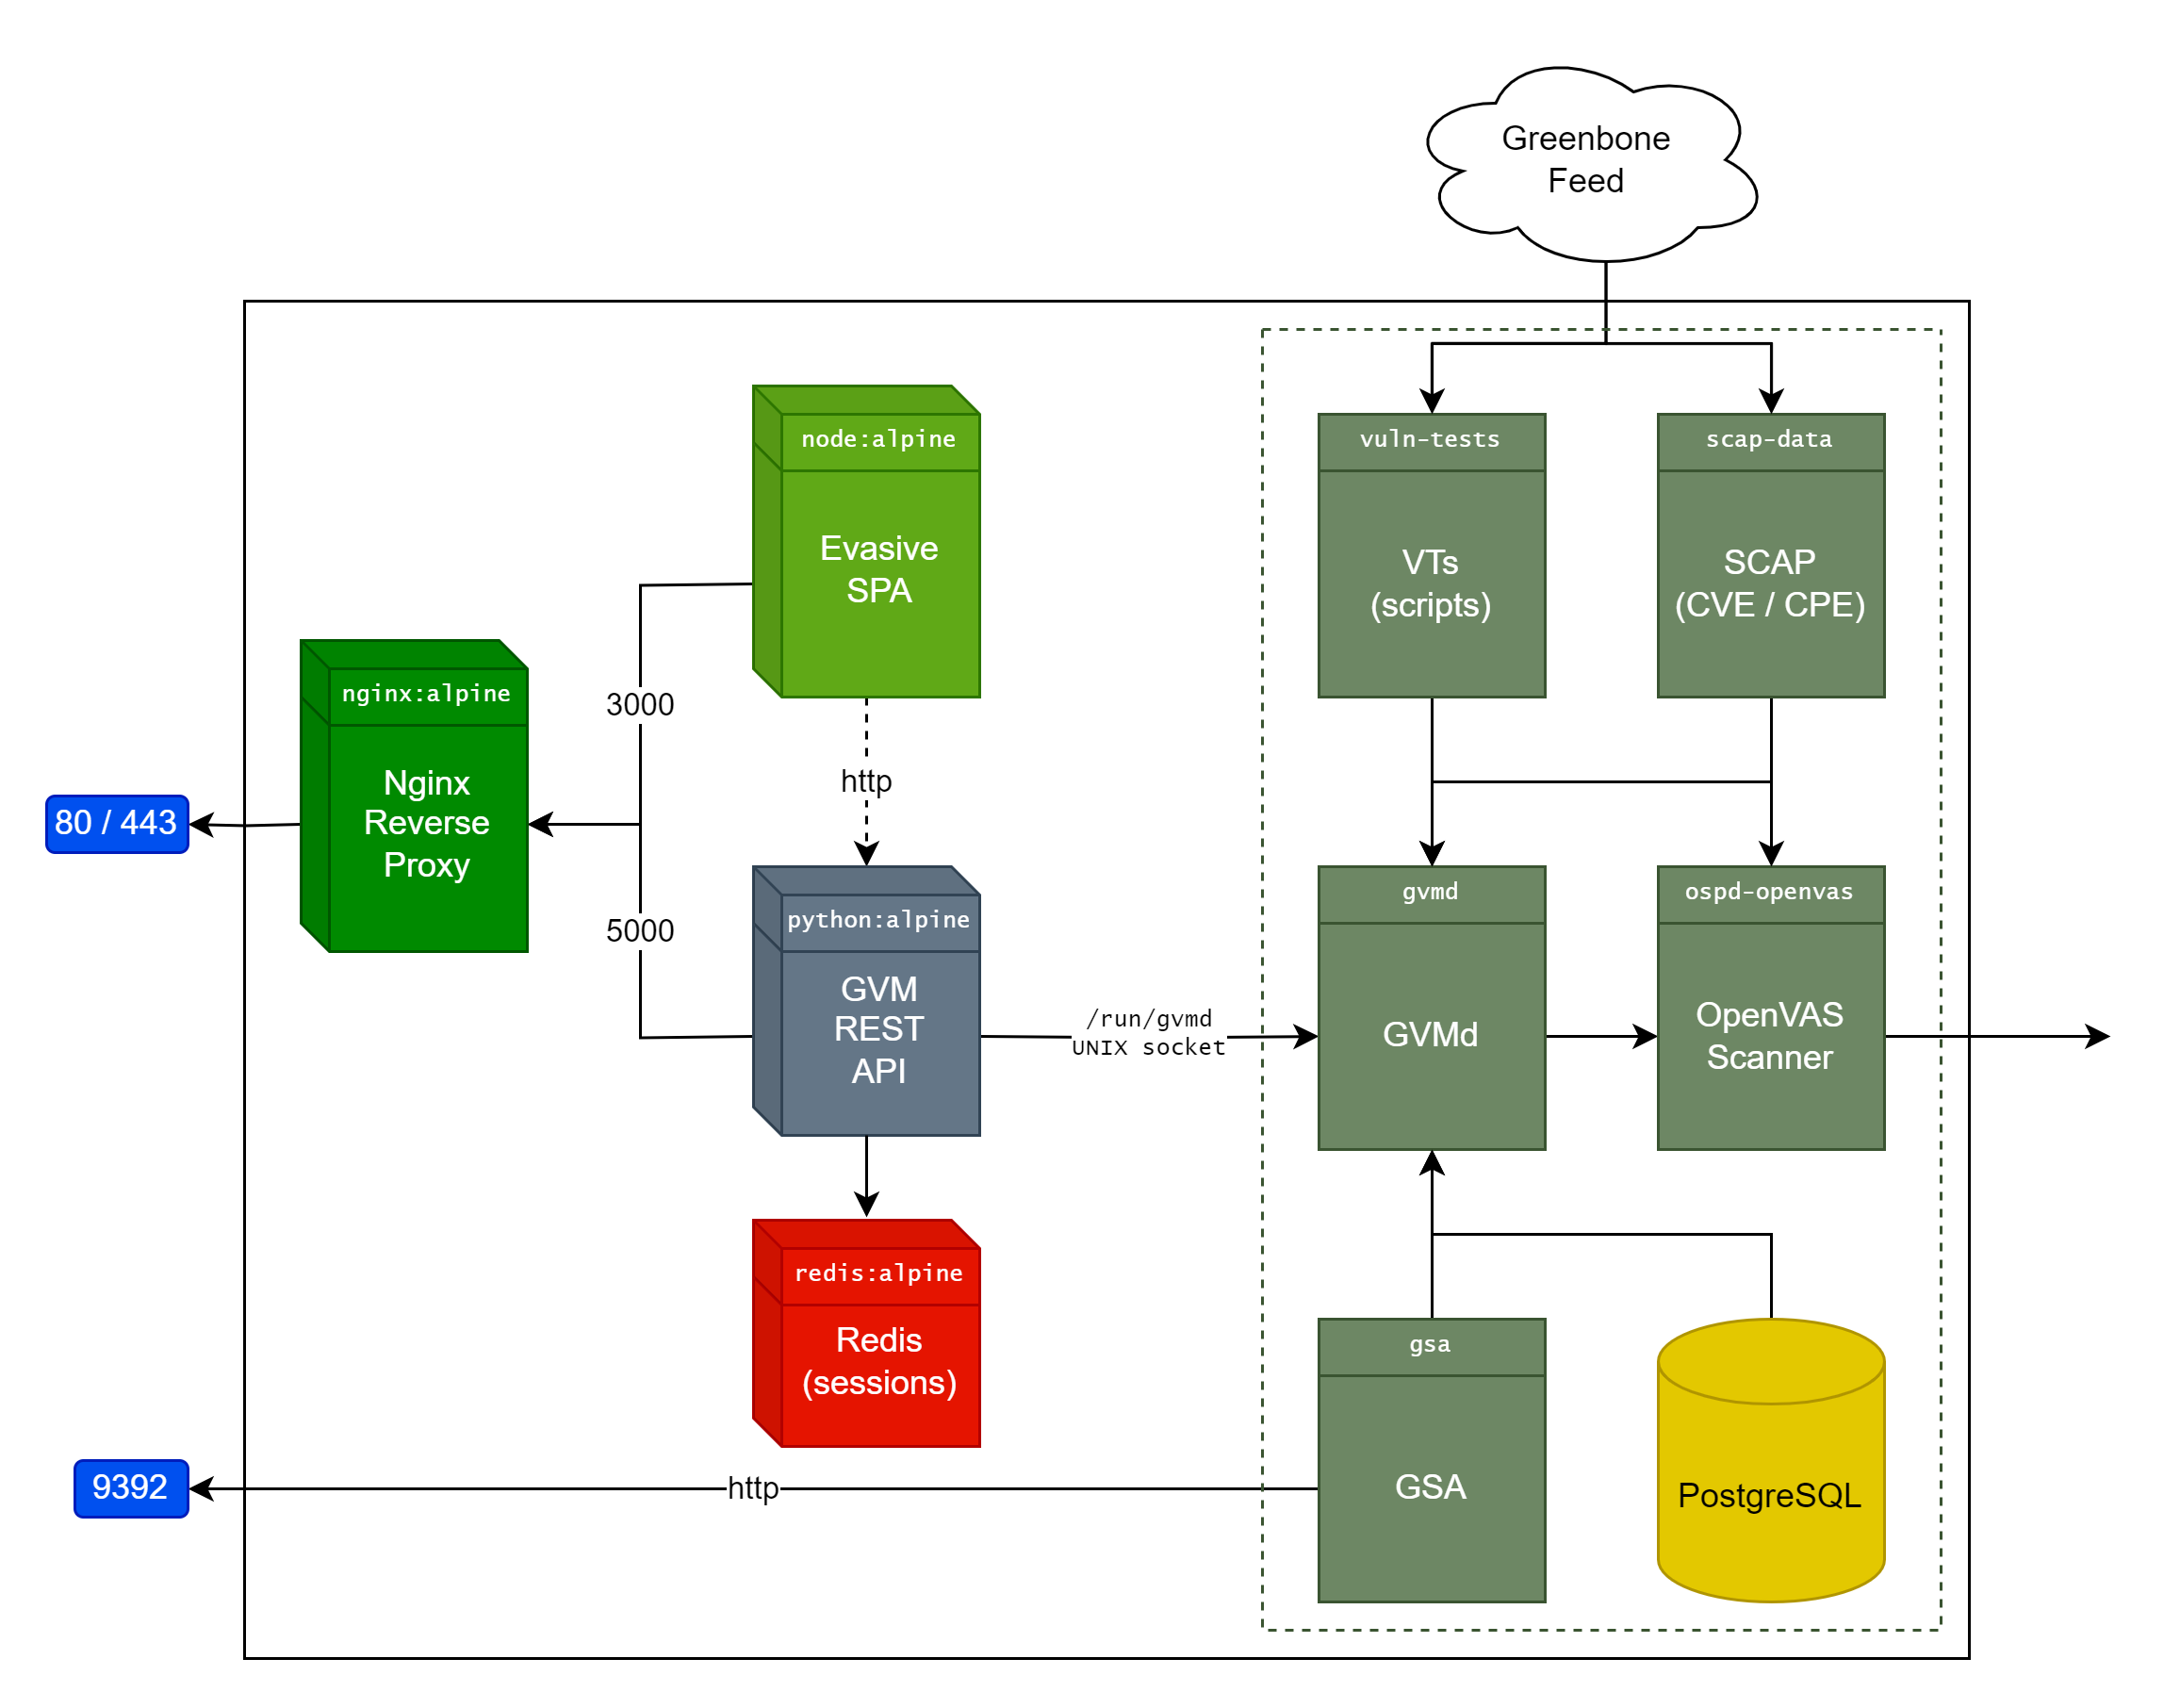
\includegraphics[width=\textwidth]{img/systems.png}
    \caption{Struttura generale dei container specificati con Docker Compose, nonché delle principali interconnessioni con il sistema Greenbone. Si noti che il framework Greenbone contiene molti più componenti di quelli elencati nel grafico, di cui molti utilizzati \emph{una tantum} dallo stesso framework. L'interconnessione centrale con il sistema Greenbone (tratteggiato) avviene mediante un volume Docker condiviso tra il container del demone GVM e il container del backend Flask. Sono presenti anche altri volumi Docker usati per la persistenza di altri dati in ambo le parti (es. le sessioni di Redis e PostgreSQL), ma non sono stati riportati nel diagramma per leggibilità.}
    \label{fig:architecture}
\end{figure}